\documentclass[12pt]{article}
\usepackage{amssymb,amsmath,graphicx,mathtools}
\usepackage{listings}
\usepackage[margin=0.75in]{geometry}
\parindent 16 pt
\usepackage{fancyhdr}
\pagestyle{fancy}
\fancyhead[R]{Swupnil Sahai}
\fancyhead[L]{Square Root Hierarchical Model}
\DeclarePairedDelimiter\ceil{\lceil}{\rceil}
\DeclarePairedDelimiter\floor{\lfloor}{\rfloor}

\lstset{
    language=R,
    basicstyle=\scriptsize\ttfamily,
    stepnumber=1,
    numbersep=5pt,
    showspaces=false,
    showstringspaces=false,
    showtabs=false,
    frame=single,
    tabsize=2,
    captionpos=b,
    breaklines=true,
    breakatwhitespace=false,
    escapeinside={},
    keywordstyle={},
    morekeywords={}
    }

\begin{document}

% CUSTOM SHORTCUTS

\def\ci{\perp\!\!\!\perp}
\def\ex{\mathbb{E}}
\def\prob{\mathbb{P}}
\def\ind{\mathbb{I}}
\def\grad{\triangledown}
\def\bigo{\mathcal{O}}

\section{General Model Framework}
We wish to split the sky map into longitudinal bins, regressing FUV ($y_{ij}$) on i100 ($x_{ij}$) within each bin $i$. As such, this problem lends itself to a hierarchical framework in which each longitudinal bin has its own slope $\beta_i$ and intercept $\alpha_i$, which are both linear functions of the light intensity ($f_i$) of the bin. This can be represented graphically as:\\

\indent\indent\indent\indent\indent\indent\indent\indent 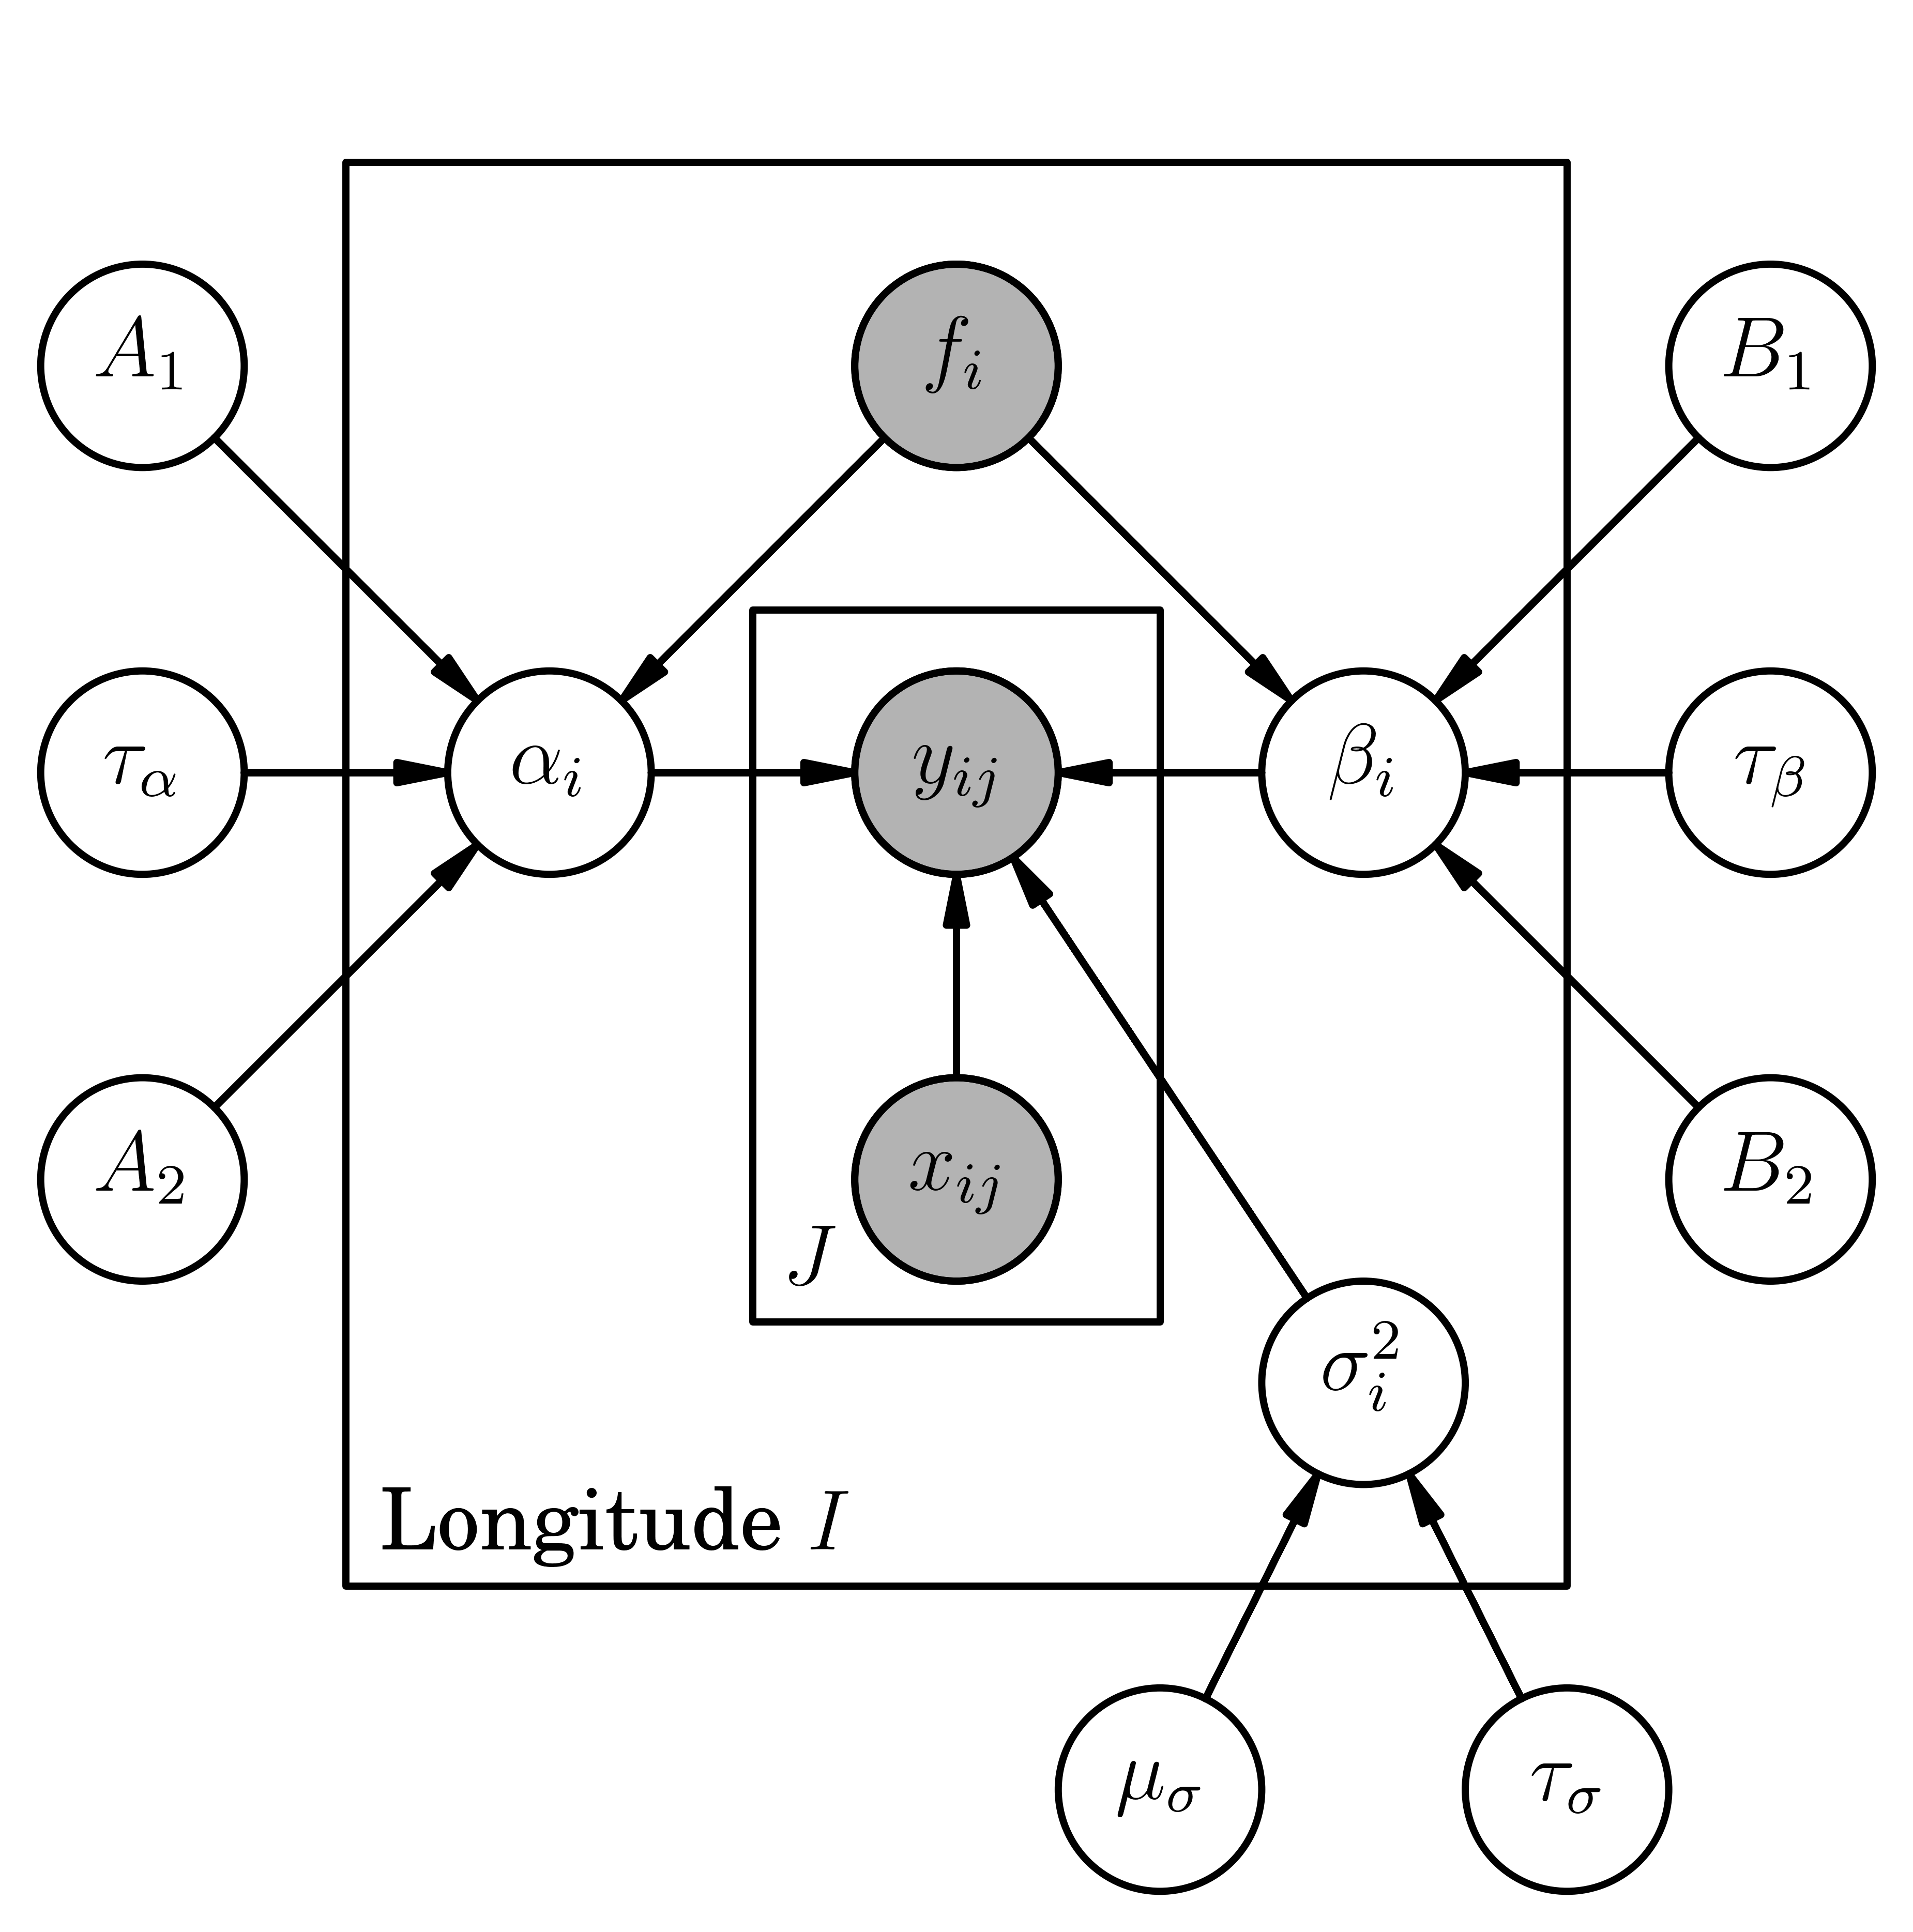
\includegraphics{LightIntensity_Model.png}

\subsection{Linear Model}
We model $y_{ij}$ as a square root function of the strictly positive parameters with the following setup:
$$y_{ij} \sim N \biggl( \alpha_i + \beta_i x_{ij} , \sigma_i^2 \biggr)
\hspace{20 pt} \alpha_i \sim N(A_1 + A_2 f_i, \tau_\alpha)
\hspace{20 pt} \beta_i \sim N(B_1 + B_2 f_i, \tau_\beta)
\hspace{20 pt} \log\sigma_i \sim N(\mu_\sigma,\tau_\sigma^2)$$

\subsection{Square Root Model}
We model $y_{ij}$ as a square root function of the strictly positive parameters with the following setup:
$$y_{ij} \sim N \biggl( \sqrt{ \alpha_i^2 + \beta_i^2 x_{ij}^2} , \sigma_i^2 \biggr)
\hspace{20 pt} \alpha_i \sim N(A_1 + A_2 f_i, \tau_\alpha)
\hspace{20 pt} \beta_i \sim N(B_1 + B_2 f_i, \tau_\beta)
\hspace{20 pt} \log\sigma_i \sim N(\mu_\sigma,\tau_\sigma^2)$$


\pagebreak
\section{Linear Model Fitting}
We fit the model with 360 bins (100 data points sampled from each bin, with i100 bounded above by 4) and four chains of 1000 iterations (4.29 minutes).\\

\noindent Strangely, the four chains for the hyper parameters $A_1, A_2, B_1,$ and $B_2$ are not mixing.

 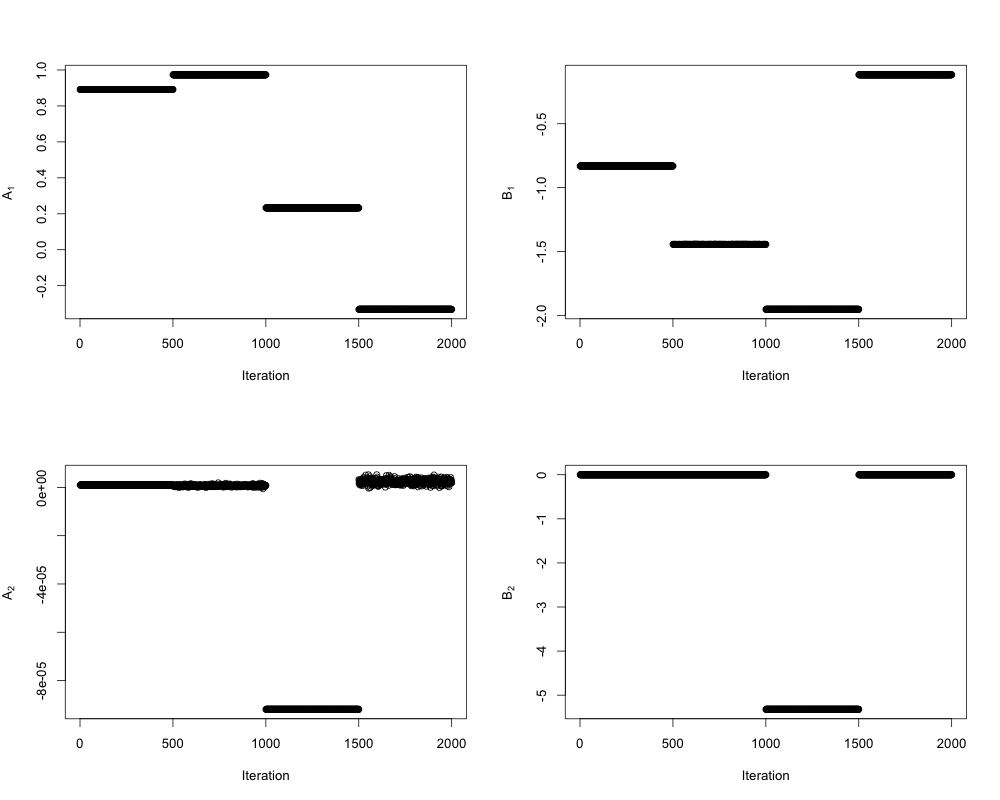
\includegraphics[scale=0.5]{HyperParams.png}

\pagebreak
\section{Square Root Model Fitting}
The same issue is present when we fit the square root model.

 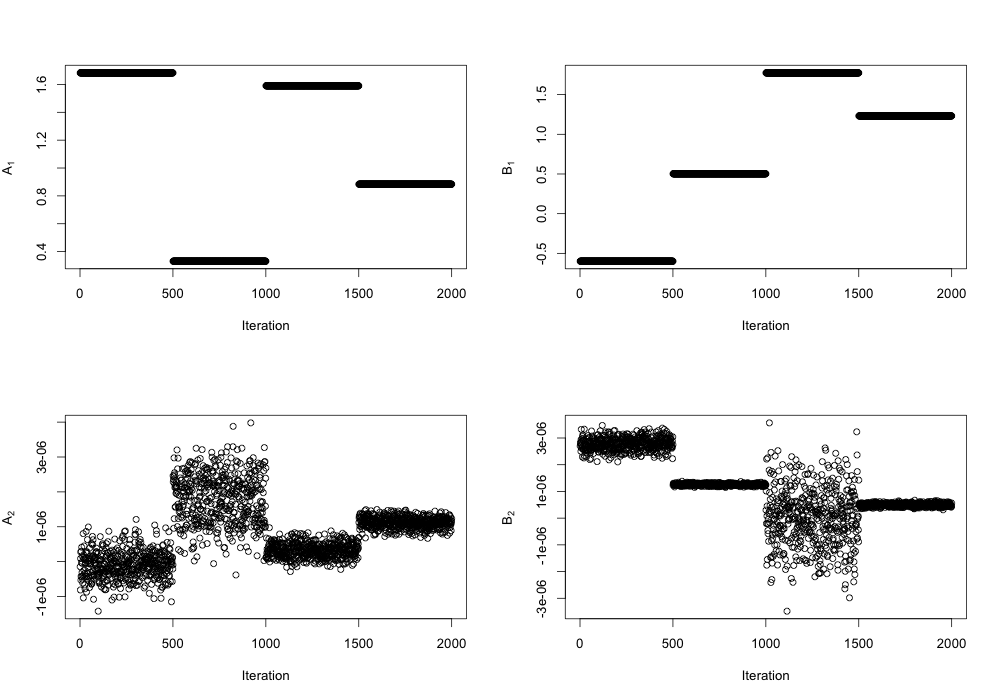
\includegraphics[scale=0.5]{HyperParams2.png}
%CODE
%\pagebreak
%\section{Code}
%\texttt{\lstinputlisting{hierarchical_model.R}}

\end{document}